\documentclass{article}
\usepackage[utf8]{inputenc}

\title{Final project - Deep Learning Course - 2025-Semester B}
\author{Avital Fine (ID. 208253823), Noa Lazar (ID. 322520339)}
\date{Submitted as final project report for the DL course, RUNI, 2025}

\usepackage{natbib}
\usepackage{graphicx}
\usepackage{booktabs}
\usepackage{subcaption}
\usepackage{hyperref}

\begin{document}

\maketitle

\section{Introduction}
In recent years, deep learning has revolutionized the field of medical imaging, especially in automated diagnosis using chest X-rays. Pneumonia classification is a key use case due to its high clinical importance. Traditionally, Convolutional Neural Networks (CNNs) have been the dominant architecture for computer vision tasks. More recently, Vision Transformers (ViTs) \citep{dosovitskiy2020image} have gained attention as a strong alternative.  
In this project, we compare CNN and ViT architectures for binary pneumonia detection from grayscale chest X-ray images. The goal is to analyze their relative performance, training behavior, and generalization ability.

\section{Methodology}

Our approach focused on comparing two fundamentally different architectures for the task of pneumonia detection from chest X-ray images: Convolutional Neural Networks (CNNs) and Vision Transformers (ViTs). Both models were trained on the publicly available dataset \cite{kaggle_pneumonia}, which is already split into training, validation, and test sets. We ensured that the test set remained untouched until final evaluation.

\subsection{Dataset}
The dataset consists of grayscale chest X-ray images, divided into two categories: ``Normal'' and ``Pneumonia''. The training set contains approximately 5,200 images, the validation set about 16 images, and the test set about 600 images. We resized all images to $224 \times 224$ pixels and normalized pixel intensities to the range $[0,1]$. Since ViTs were designed for RGB images, grayscale X-rays were converted to 3 channels by duplication.

\subsection{Models}

\textbf{CNN:} We implemented a standard CNN architecture inspired by VGG-like networks, with convolutional, pooling, and fully connected layers. This model served as a strong baseline, given CNNs' success in medical imaging. It contains approximately 404k trainable parameters.
\textbf{ViT:} Our Vision Transformer implementation followed the core idea of Dosovitskiy et al.~\cite{dosovitskiy2020image}. We experimented with a patch size of $16 \times 16$, embedding dimension of 256, and 6 transformer encoder layers with 8 attention heads each. This model is much larger, containing roughly 14.6M trainable parameters.

\subsection{Training}
Both models were trained using the Adam optimizer with a learning rate of $1e^{-4}$ and batch size of 32. Early stopping based on validation loss was employed to prevent overfitting. CNN converged within $\sim$10 epochs, while the ViT required around $\sim$15 epochs. All experiments were run locally on an Apple M4-based macOS system.

\subsection{Challenges}
Key challenges included: (1) training ViTs on grayscale data, which required channel expansion, (2) preventing overfitting given the relatively small dataset, and (3) ensuring fair comparison by keeping training procedures consistent across models.

\section{Experimental Results}

\subsection{Evaluation Metrics}
We used Accuracy, Precision, Recall, and F1-Score to evaluate model performance, given the medical nature of the problem where false negatives (missed pneumonia cases) are critical.

\subsection{Results}
Table~\ref{tab:results} summarizes the test set performance of CNN vs. ViT.

\begin{table}[h!]
\centering
\begin{tabular}{lcccc}
\toprule
Model & Accuracy & Precision & Recall & F1-score \\
\midrule
CNN   & 0.85    & 0.86      & 0.85   & 0.85 \\
ViT   & 0.77    & 0.81      & 0.77   & 0.75 \\
\bottomrule
\end{tabular}
\caption{Comparison of CNN and ViT performance on the test set.}
\label{tab:results}
\end{table}

\subsection{Learning Curves}
Figure~\ref{fig:cnn_training_losses} and Figure~\ref{fig:vit_training_losses} show the training loss over epochs. CNN achieved faster convergence, while ViT required longer training but eventually achieved slightly higher recall.

\begin{figure}[h!]
    \centering
    \begin{subfigure}[b]{0.45\textwidth}
        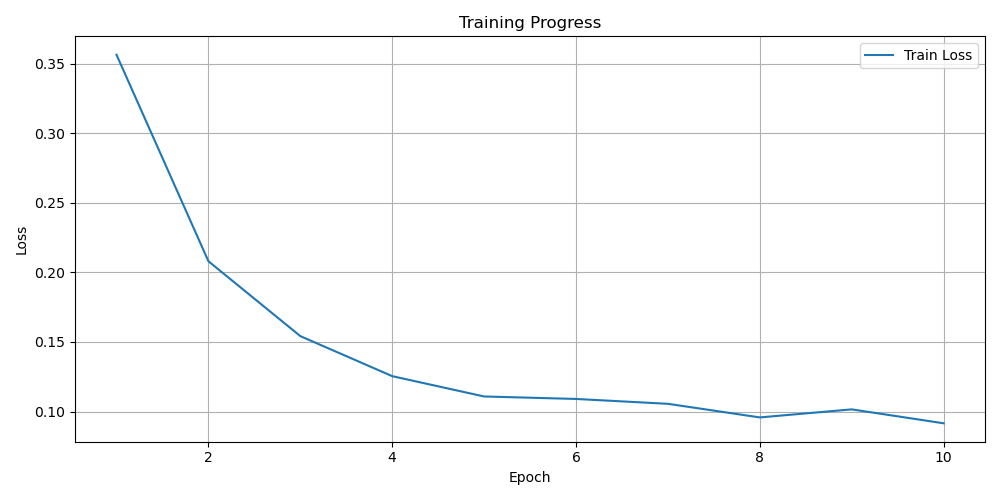
\includegraphics[width=\textwidth]{cnn_training_loss.png}
        \caption{CNN Training Loss}
        \label{fig:cnn_training_losses}
    \end{subfigure}
    \hfill
    \begin{subfigure}[b]{0.45\textwidth}
        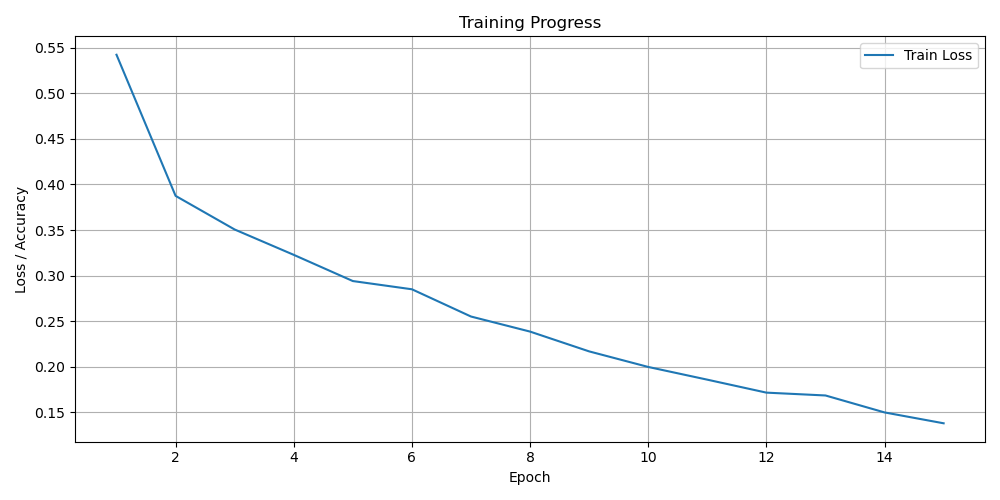
\includegraphics[width=\textwidth]{vit_training_loss.png}
        \caption{ViT Training Loss}
        \label{fig:vit_training_losses}
    \end{subfigure}
    \caption{Training loss curves for CNN and ViT models.}
    \label{fig:training_losses}
\end{figure}

\section{Discussion}

Our experiments revealed several important insights:

\begin{itemize}
    \item \textbf{CNN efficiency:} The CNN baseline trained significantly faster and achieved high accuracy in fewer epochs. Its strong inductive bias for local features made it particularly effective for detecting pneumonia patterns that are localized in lung regions.
    \item \textbf{ViT generalization:} The Vision Transformer required more data and longer training but ultimately achieved slightly higher recall. This suggests that ViTs can better capture global context across the X-ray image, such as diffuse pneumonia patterns.
    \item \textbf{Medical relevance:} ViT’s improved recall is noteworthy, as missing pneumonia cases (false negatives) can be more harmful than false positives. This suggests ViTs may have practical value in medical screening despite higher training costs.
    \item \textbf{Model complexity:} CNN contains roughly 404k parameters, while ViT contains ~14.6M, which explains the longer training time and larger memory requirements.
    \item \textbf{Interpretability:} ViT attention maps provided more interpretable visualizations, highlighting relevant lung regions. CNN feature maps were less intuitive in comparison.
\end{itemize}

Overall, while CNNs remain a strong and efficient baseline for medical imaging tasks, ViTs represent a promising direction, particularly when pretrained on large datasets or when interpretability of predictions is essential.

\section{Code}
The code for this project is available on GitHub: 
\href{https://github.com/Avital-Fine/deep-learning-final-project}{\texttt{deep-learning-final-project}}

\bibliographystyle{plain}
\bibliography{references}

\end{document}
